% !TEX root = ../Thesis.tex

\chapter{Gestione della memoria}
Questo capitolo esplorerà nel dettaglio come Java e Rust affrontano il tema della gestione della memoria. Entrambi i linguaggi, a differenza di C/C++, sollevano il programmatore dalla responsabilità di gestire manualmente la deallocazione della memoria, adottando però filosofie e approcci differenti:
\begin{itemize}
    \item Java affida al \textit{Garbage Collector (GC)} il compito di liberare la memoria automaticamente, semplificando lo sviluppo ma introducendo overhead. 
    \item Rust elimina il GC grazie a un sistema di \textit{ownership} e \textit{borrowing}, garantendo deallocazione deterministica e sicurezza a compile-time. 
\end{itemize}
\section{L'approccio di Java}
Java è un linguaggio di programmazione progettato per essere semplice, portabile e sicuro, con una gestione della memoria che mira a ridurre la complessità e prevenire errori comuni legati all'uso diretto delle risorse. Java raggiunge questi obiettivi affidando l'intera gestione della memoria alla Java Virtual Machine (JVM). Gli aspetti fondamentali dell'approccio Java sono:

\begin{enumerate}
\item L'allocazione automatica della memoria tramite JVM: gli oggetti vengono creati dinamicamente nell'heap senza che il programmatore debba preoccuparsi di allocare la memoria manualmente. 
\item La deallocazione automatica della memoria tramite il garbage collector, una componente della JVM che si occupa di individuare e liberare la memoria occupata da oggetti non più raggiungibili, prevenendo così problemi comuni in altri linguaggi, come memory leak e dangling pointer\footnote{Un dangling pointer è un riferimento a una variabile che è stata deallocata e quindi non più valido.}. Questo, di fatto, toglie al programmatore la responsabilità collegata al dover gestire manualmente la deallocazione della memoria, riducendo la probabilità di errori nel codice.
\item La prevenzione di comportamenti indefiniti a run-time, attraverso un controllo rigoroso dell'accesso alla memoria a runtime: ad esempio, accessi a riferimenti \texttt{null} generano eccezioni gestibili da parte dello sviluppatore. 
\end{enumerate}

Tuttavia, l'approccio automatico della gestione della memoria porta alcuni svantaggi per quanto riguarda le prestazioni del programma. Il garbage collector, infatti, introduce un overhead significativo, poiché deve periodicamente eseguire la scansione della memoria per identificare gli oggetti non più raggiungibili e liberare la memoria occupata da essi. Questo processo può causare pause impreviste nell'esecuzione del programma, che possono essere problematiche quando si richiedono alte prestazioni. La JVM moderna implementa algoritmi di garbage collection avanzati \cite{dynatrace-gc-pause} per cercare di ridurre al minimo le interruzioni e ottimizzare le prestazioni, ma il costo di queste operazioni rimane comunque un fattore da considerare. 

È importante sottolineare, inoltre, che, nonostante il garbage collector riduca notevolmente il rischio di errori di memoria, non elimina completamente la possibilità di \textit{memory leak} \cite{baeldung-java-memory-leaks}. Un memory leak in Java si verifica quando un oggetto non più necessario continua a essere referenziato, impedendo al garbage collector di liberare la memoria da esso occupata. Alcuni casi più comuni di memory leak in Java includono:
\begin{itemize}
    \item Memory leak causati da campi dichiarati come \texttt{static}. In Java, i campi \texttt{static} sono associati alla classe e non all'istanza, quindi rimangono in memoria finché la classe è caricata dalla JVM. Questo, solitamente, coincide con l'intero ciclo di vita dell'applicazione. Ad esempio: 
    \begin{minted}[fontsize=\small]{Java}
    public class MemoryLeakExample {
        private static List<String> list = new ArrayList<>();

        public static void populateList() {
            for (int i = 0; i < 1000000; i++) {
                list.add("Item " + i);
            }
        }

        public static void main(String[] args) {
            new MemoryLeakExample().populateList();
        }
    }
    \end{minted}
    In questo caso, una volta che il metodo \texttt{populateList()} termina la sua esecuzione, la memoria occupata da \texttt{list} non viene liberata, poiché è un campo \texttt{static}. Questo non si verifichrebbe se \texttt{list} fosse una variabile d'istanza, poiché la memoria da essa occupata verrebbe liberata quando l'istanza della classe viene raccolta dal garbage collector.
    \item Memory leak causati da risorse non chiuse correttamente. In Java, oggetti che si riferiscono a risorse di sistema, come file o connessioni di rete, devono essere chiusi esplicitamente per liberare la memoria e le risorse associate. In caso contrario, possono causare memory leak. Ad esempio:
    \begin{minted}[fontsize=\small]{Java}
    public class MemoryLeakExample {
        public static void main(String[] args) {
            try {
                Scanner sc = new Scanner(new File("file.txt"));
                // Logica di utilizzo dello Scanner
            } catch (FileNotFoundException e) {
                e.printStackTrace();
            }
            // Memory leak causato dallo Scanner non chiuso
        }
    }
    \end{minted}
\end{itemize}

\section{L'approccio di Rust}
Rust è un linguaggio di programmazione moderno progettato per garantire sicurezza nella gestione della memoria senza fare uso di un garbage collector. Rust ha due obiettivi principali:
\begin{enumerate}
    \item  Garantire che il programma sia privo di comportamenti indefiniti, ovvero situazioni in cui il programma può agire in modo imprevedibile. Un esempio tipico è l'accesso a memoria non valida, che può portare all'esecuzione di codice con dati non inizializzati o causare errori di memoria come segmentation fault. 
    \item Eseguire la prevenzione di comportamenti indefiniti a compile-time, piuttosto che a run-time. Questo significa che il compilatore di Rust è in grado di rilevare e segnalare errori di memoria prima che il programma venga eseguito, riducendo il rischio di bug e di errori durante l'esecuzione. 
    % Nell'articolo di google viene riportato il vantaggio di non avere controlli a run-time.
\end{enumerate}
L'approccio di Rust consente di evitare interamente classi di errori comuni nei linguaggi tradizionali: buffer overflow, dangling pointer e race condition sui dati condivisi. Inoltre, poiché questi controlli vengono effettuati a compile-time, Rust riduce drasticamente la necessità di controlli a run-time, migliorando le prestazioni senza sacrificare la sicurezza. 

Rust non può prevenire tutti i possibili bug relativi alla gestione della memoria ma le metodologie messe in atto rendono i programmi scritti in Rust significativamente più sicuri rispetto a quelli sviluppati in linguaggi con meno controlli. Un esempio concreto è fornito da Google \cite{android13-memorysafe}, che ha introdotto il linguaggio nello sviluppo di Android 13. In particolare, circa il 21\% del nuovo codice introdotto in Android 13 è stato scritto in Rust, e, alla data della pubblicazione dell'articolo, non sono state scoperte vulnerabilità di sicurezza legate alla memoria in questo codice. Questo è un risultato significativo che dimostra come gli obiettivi prefissati dagli sviluppatori di Rust siano stati raggiunti nella pratica.

Rust realizza questi obiettivi attraverso un sistema basato sui concetti di \textit{ownership} (proprietà) e \textit{borrowing} (prestito). Concetti fondamentali che verrano affrontati in dettaglio nelle prossime sezioni.

\section{Stack e Heap}
Sia Java che Rust utilizzano due aree di memoria principali: lo stack e l'heap, ma la loro gestione è profondamente diversa, riflettendo i diversi modelli di memoria adottati dai due linguaggi.

Lo stack è un'area di memoria strutturata secondo una struttura dati stack LIFO (Last In, First Out). La memoria stack è contigua e i dati memorizzati al suo interno sono in posizione fissa rispetto allo stack pointer, un puntatore che punta all'ultimo elemento inserito. Questo permette un accesso rapido ai dati usando indirizzi di memoria calcolati in modo semplice tramite un offset rispetto allo stack pointer. Inoltre, allocazione e deallocazione della memoria stack sono molto veloci poiché avvengono spostando lo stack pointer, avanti o indietro, di un numero di byte opportuno rispetto alla dimensione del dato e all'architettura della CPU.

L'heap, al contrario, è un'area di memoria in cui i dati possono essere allocati in qualsiasi sua posizione. L'allocazione e la deallocazione della memoria heap richiedono operazioni più complesse rispetto allo stack, poiché il sistema operativo deve tenere traccia degli spazi liberi e occupati. Questo può portare a un utilizzo meno efficiente della memoria (frammentazione) e a un accesso più lento ai dati rispetto allo stack. 

In Java, l'allocazione della memoria è fortemente automatizzata. Ogni volta viene creato un oggetto, tramite la keyword \texttt{new}, viene allocata dinamicamente memoria heap nel quale sarà memorizzato l'oggetto. L'uso dello stack è limitato a variabili di tipo primitivo e variabili locali. Al contrario, Rust adotta un modello più esplicito e flessibile. In Rust, la variabili possono essere allocate sia nello stack che nell'heap, a seconda dalla conoscenza a compile time delle dimensioni del dato:
\begin{itemize}
    \item  Se la variabile ha una dimensione fissa nota a compile time, viene allocata nello stack. È possibile allocare nell'heap anche variabili di dimensione fissa attraverso \texttt{Box}\footnote{\texttt{Box<T>} è uno smart pointer fornito dalla standard library di Rust che consente di allocare un valore di tipo \texttt{T} sull'heap.}.
    \item  Se la variabile ha una dimensione variabile o non nota a compile time, viene allocata nell'heap. 
\end{itemize} 
Questa è una differenza fondamentale rispetto a Java, perchè permette allo sviluppatore di avere più controllo su dove vengono allocati i dati, permettendo ottimizzazioni specifiche per le esigenze del programma. 

Ad esempio, sia in Java che in Rust, gli array hanno una dimensione fissa. Tuttavia, in Java, gli array sono allocati nell'heap e sono referenziati da variabili nello stack, mentre in Rust, poiché si conosce la loro dimensione a compile time, vengono allocati nello stack. Questo rende l'accesso agli elementi dell'array di Rust più veloce. 
\begin{minted} [fontsize=\small] {Java}
    int[] arr = {1, 2, 3, 4, 5}; // Array allocato nell'heap
    System.out.println("Il primo elemento e': " + arr[0]);
\end{minted}
\begin{minted} [fontsize=\small] {Rust}
    let arr = [1, 2, 3, 4, 5]; // Array allocato nello stack
    println!("Il primo elemento e': {}", arr[0]);
\end{minted}
\section{Ownership}
L'ownership è un concetto fondamentale di Rust il quale può essere definito come un insieme di regole che il compilatore controlla per garantire una corretta gestione della memoria. Questo significa sia garantire che non ci siano errori di memoria a run-time, sia che la memoria inutilizzata venga rilasciata correttamente per non terminare lo spazio di memoria disponibile. 

L'obiettivo principale dell'ownership è, quindi, quello di gestire la memoria heap tenendo traccia di quali parti di codice utilizzano valori contenuti in essa, minimizzare valori duplicati e garantire che la memoria venga rilasciata quando non è più necessaria. 
%TODO: Forse inserire confronto con Java su performance e garbage collector 

L'ownership si basa su tre regole principali: 
\begin{enumerate}
    \item  Ogni valore in Rust ha un \textit{owner} (proprietario), ovvero una variabile che ne detiene la proprietà. 
    \item  Un valore può avere un solo owner alla volta. 
    \item  Quando l'owner di un valore esce dallo scope, il valore viene automaticamente rilasciato dalla memoria.
\end{enumerate}
Consideriamo un caso banale in cui si crea una variabile all'interno di uno scope:
\begin{minted} [fontsize=\small] {Rust}
    {
        let s = String::from("Hello");
    }
\end{minted}
In questo caso, secondo la regola 3, quando la variabile \texttt{s} esce dallo scope, il valore \texttt{"Hello"} viene automaticamente rilasciato dalla memoria. Questo avviene attraverso la funzione \texttt{drop} che viene chiamata automaticamente da rust nel momento in cui la variabile esce dallo scope. In Java questo non accade. Dato il seguente codice equivalente in Java:
\begin{minted} [fontsize=\small] {Java}
    {
        String s = new String("Hello");
    }
\end{minted}
La memoria occupata dalla stringa \texttt{"Hello"} non viene rilasciata automaticamente quando \texttt{s} esce dallo scope, ma solo quando il garbage collector esegue la raccolta dei valori non più raggiungibili. Già da questo semplice caso si può notare come l'ownership di Rust permetta di avere un controllo più preciso sulla memoria. 

Un altro aspetto importante dell'ownership è che, quando si assegna un valore a un'altra variabile, l'ownership viene trasferita. Ad esempio, consideriamo il seguente codice:
\begin{minted} [fontsize=\small] {Rust}
    let s1 = String::from("Hello");
    let s2 = s1; // Ownership di s1 viene trasferita a s2
    println!("{}", s1); // Errore di compilazione
    println!("{}", s2);
\end{minted}
\begin{figure}[h]
    \centering
    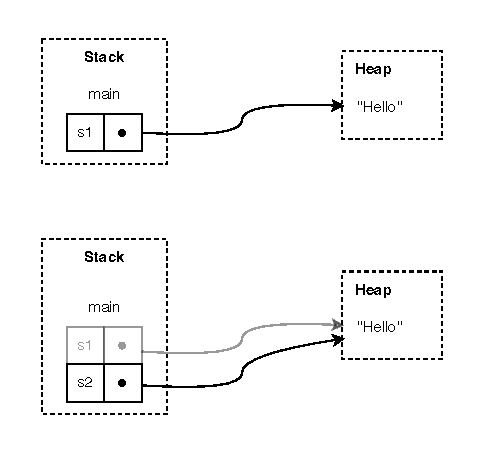
\includegraphics[scale = 1]{Figures/own1.drawio.pdf}
    \caption{Visualizzazione memoria Rust dopo il trasferimento di ownership.}
    \label{fig:own1}
\end{figure}
In questo caso, l'ownership della stringa \texttt{"Hello"} viene trasferita da \texttt{s1} a \texttt{s2}. Come si può vedere in figura \ref{fig:own1}, dopo il trasferimento, \texttt{s1} non è più valida e qualsiasi tentativo di accedervi causerà un errore di compilazione.

In Rust, per variabili il cui valore è contenuto in memoria heap, un'istruzione di copia esegue una \textit{shallow copy} del valore e invalida la variabile originale. Questo comportamento prende il nome di \textit{move}. L'operazione di move è a tutti gli effetti come un trasferimento di proprietà legale, dove il vecchio proprietario non può più accedere alla proprietà venduta. Rust non esegue mai una \textit{deep copy} di una variabile: se il programmatore desidera duplicare effettivamente il contenuto, deve farlo in modo esplicito (ad esempio usando il metodo \texttt{clone()}). Quindi, l'operazione di copia base è poco costosa in termini di performance.

Questo non è consistente con quello che accade in Java, dove l' assegnazione di un oggetto a un'altra variabile non invalida quella originale, ma crea una nuova referenza all'oggetto esistente. Entrambe le variabili possono accedere all'oggetto, condividendone lo stato. In Java, il codice equivalente sarebbe:
\begin{minted} [fontsize=\small] {Java}
    String s1 = "Hello";
    String s2 = s1; 
    System.out.println(s1); // Valido
    System.out.println(s2); // Valido
\end{minted}
In questo caso, quindi, entrambe le stringhe verrebbero correttamente stampate. L'approccio adottato da Rust è decisamente più restrittivo, ma si tratta di una caratteristica desiderabile: consente infatti di evitare errori comuni legati alla gestione della memoria, come l'accesso a variabili non più valide o la modifica involontaria di dati condivisi. 
\subsubsection {Ownership e funzioni}
Il meccanismo di passaggio degli argomenti a funzione in Rust è strettamente legato al concetto di ownership. Quando si passa una variabile a una funzione, l'ownership di quella variabile viene trasferita alla funzione, rendendo, quindi, la variabile originale non più utilizzabile dopo la chiamata. Questo avviene perché Rust utilizza il \textit{pass-by-value}. Ad esempio, consideriamo il seguente codice:
\begin{minted} [fontsize=\small] {Rust}
    fn main() {
        let s1 = String::from("Hello");
        // Ownership di s1 viene trasferita a print_string
        print_string(s1); 
        println!("{}", s1); // Errore di compilazione
    }

    fn print_string(s: String) {
        println!("{}", s);
    }       
\end{minted}
Ciò che accade è: la variabile \texttt{s1} viene passata alla funzione \texttt{print\_string}, ossia \texttt{s1} viene copiata in \texttt{s} e, quindi, l'ownership dei dati di \texttt{s1} passa a \texttt{s}. Come risultato, \texttt{s1} non è più valida dopo la chiamata alla funzione, e qualsiasi tentativo di accedervi causerà un errore di compilazione. 

Java, come Rust, utilizza il \textit{pass-by-value}, ma il passaggio di un oggetto a una funzione non invalida la variabile originale, questo può portare a situazioni sgradevoli.
\begin{listing}[h]
    \begin{minted} [fontsize=\small] {Java}
        class Person {
            private String name;
            public Person(String name) {
                this.name = name;
            }

            public void setName(String name) {
                this.name = name;
            }

            public String getName() {
                return name;
            }
        }

        public class Main {
            public static void main(String[] args) {
                Person p1 = new Person("Alice");
                Person p2 = p1;
                p2.setName("Bob"); // Modifica il nome di p1 e p2
                System.out.println(p1.getName()); // Stampa "Bob"
            }
        }
    \end{minted}
    \caption{Modifica di un oggetto tramite un riferimento in Java.}
    \label{lst:java-reference}
\end{listing}
Nel listato \ref{lst:java-reference}, la modifica del campo \texttt{name} di \texttt{p2} influisce anche \texttt{p1}, poiché entrambi i riferimenti puntano allo stesso oggetto in memoria. Questo comportamento può causare bug sottili e difficili da individuare, specialmente in contesti complessi o concorrenti\footnote{È utile notare che, in Java, la keyword \texttt{final} può essere utilizzata per dichiarare una variabile come immutabile. Tuttavia, \texttt{final} non rende immutabile l'oggetto a cui la variabile si riferisce: i campi dell'oggetto possono ancora essere modificati tramite metodi mutator.}. In Rust, invece, il trasferimento di ownership impedisce il comportamento appena descritto, poiché, una volta che l'ownership è stata trasferita, la variabile originale non può più essere utilizzata.

\begin{quote}
    Some people say that Java uses “call by reference” for objects. In a language that supports call by reference, a method can replace the contents of variables passed to it. In Java, all parameters—object references as well as primitive type values—are passed by value.
\end{quote}
\begin{flushright}
--- Cay S. Horstmann \cite{horstmann-java-impatient}
\end{flushright}

È importante sottolineare che la semantica del \textit{move} in Rust, così come descritta finora, si applica ai tipi di dati che allocano memoria sull'heap, come \texttt{String} o \texttt{Vec}. In questi casi, un'assegnazione o il passaggio a una funzione comporta il trasferimento dell'ownership, e quindi l'invalidazione del valore originale. Tuttavia, per tipi primitivi e a dimensione fissa, nota a compile time, come gli interi (\texttt{i32}, \texttt{u64}, etc.), Rust applica una semantica diversa: questi tipi implementano automaticamente il \texttt{trait}\footnote{Un trait definisce un insieme di metodi che un tipo può implementare. È simile a un'interfaccia Java: stabilisce un contratto che i tipi devono rispettare} \texttt{Copy}. Ciò significa che, in fase di assegnazione o di passaggio come parametro a una funzione, viene eseguita una copia bit a bit del valore, e l'ownership non viene trasferita.

Di conseguenza, entrambi i valori (l'originale e la copia) restano validi e utilizzabili, senza causare errori di compilazione. Ecco un esempio:
\begin{minted}[fontsize=\small]{rust}
    fn main() {
        let x = 42;
        print_value(x); // x viene copiato, non spostato
        println!("{}", x); // x è ancora valido
    }

    fn print_value(n: i32) {
        println!("{}", n);
    }
\end{minted}
Questa distinzione riflette chiaramente la filosofia di Rust nel garantire la sicurezza nell'accesso alla memoria:
\begin{itemize}
    \item Per i tipi che contengono dati allocati dinamicamente o che possono essere modificati a runtime, Rust usa la semantica del \textit{move}, che impedisce di accedere a un valore dopo che la sua \textit{ownership} è stata trasferita altrove, evitando così potenziali problemi di accesso concorrente e modifiche inattese.
    \item Per i tipi con dimensione fissa e nota a compile time, che risiedono interamente nello stack, solitamente immutabili per definizione (come interi o booleani)\footnote{In Rust le variabili sono immutabili a meno che non si vengano dichiarate con la keyword \texttt{mut}.}, Rust utilizza la semantica del \textit{copy}, poiché la copia bit-a-bit è efficiente e non introduce rischi di inconsistenza o accessi errati.
\end{itemize}
L'ownership può essere trasferita anche con le funzioni che ritornano un valore. In questo caso, un assegnamento a una variabile di un valore restituito da una funzione comporta il trasferimento dell'ownership dalla funzione alla variabile. Ad esempio:
\begin{minted}[fontsize=\small]{rust}
    fn main() {
        let s1 = create_string(); 
        println!("{}", s1);
    }

    fn create_string() -> String {
        String s = String::from("Hello from function")
        s // Ownership di s viene trasferita a s1
    }
\end{minted}
L'ownership di una variabile segue sempre lo stesso principio: assegnare il valore a un'altra variabile trasferisce l'ownership. Quando una variabile che include dati nell'heap esce dallo scope, il compilatore chiama automaticamente la funzione \texttt{drop} per rilasciare la memoria occupata da quei dati, a meno che l'ownership non sia stata trasferita a un'altra variabile.
\begin{listing}[H]
    \begin{minted}[fontsize=\small]{rust}
        fn main() {
            let v1 = vec![10, 20, 30];
            let (v2, sum) = sum_vector(v1); 
            println!("La somma degli elementi di {:?} è {}", v2, sum);
        }

        fn sum_vector(v: Vec<i32>) -> (Vec<i32>, i32) {
            let sum = v.iter().sum();
            (v, sum)
        }
    \end{minted}
    \caption{Trasferimento di ownership con ritorno di valore.}
    \label{lst:ownership-return}
\end{listing}

Quindi, se volessimo passare un valore a una funzione e riutilizzarlo dopo la chiamata, dovremmo ritornare quel valore al termine della funzione, eventualmente, in aggiunta ad altri valori che la funzione calcola\footnote{Questo può essere fatto tramite il tipo \texttt{Tuple}: un array di dimensione fissa in cui è possibile memorizzare dati di tipo diverso} (vedi listato \ref{lst:ownership-return}). 

\section{Borrowing}
È evidente come l'ownership sia un concetto potente per la gestione della memoria, ma che risulta troppo restrittivo e macchinoso in situazioni come quella riportata nel listato \ref{lst:ownership-return}. Rust, per risolvere questo problema, introduce il concetto di \textit{borrowing}, che consente di prendere in prestito un valore senza trasferirne l'ownership, consentendo una maggiore flessibilità. Il borrowing è realizzato attraverso il concetto di riferimento. Il riferimento in Rust non ha le stesse proprietà di un riferimento in Java: 
\begin{itemize}
    \item In Java un riferimento è l'indirizzo di memoria di un oggetto, e può essere utilizzato per accedere e modificare l'oggetto stesso. 
    
    Inoltre, può assumere il valore \texttt{null}, ossia non puntare a nessun oggetto in memoria. Questo ha gravi ripercussioni sulla sicurezza del programma, poiché l'accesso a un riferimento \texttt{null} può causare un \texttt{NullPointerException} a run-time. 
    
    Lo stesso creatore della nozione di riferimento \texttt{null}, Tony Hoare, lo ha definito "billion dollar mistake" \cite{hoare-null-reference}, a causa dei costi che le aziende devono, e dovranno, sostenere per bug e vulnerabilità dovuti a \texttt{null}.
    \item In Rust, un riferimento è anch'esso l'indirizzo di memoria di un valore (mutabile o immutabile). Tuttavia, a differenza di Java, un riferimento in Rust non può essere \texttt{null}. Il compilatore di Rust garantisce che ogni riferimento punti sempre a un valore valido di un tipo specifico per tutta la durata della sua esistenza. Questo dà importanti garanzie di sicurezza, poiché elimina la possibilità di avere errori a run-time legati a riferimenti nulli.
    %TODO: inserire come rust gestisce l'assenza di valore 
\end{itemize}
I riferimenti in Rust sono ottenuti utilizzando l'operatore di referenziazione \texttt{\&} che restituisce il riferimento alla variabile su cui viene applicato. Ad esempio:
\begin{minted}[fontsize=\small]{rust}
    fn main() {
        let s1 = String::from("Hello");
        print_string(&s1); 
    }
    fn print_string(s2: &String) {
        println!("{}", s2);
    }
\end{minted} 
In questo esempio, \texttt{s1} è una variabile che si trova nello stack e contiene un valore allocato nell'heap. Pertanto, quando si applica l'operatore \texttt{\&} a \texttt{s1}, si ottiene un riferimento a una variabile sullo stack. Quindi, come mostrato in figura \ref{fig:bor1}, si hanno due livelli di indirezione: \texttt{s2} per poter accedere a \texttt{"Hello"} deve prima seguire il riferimento a \texttt{s1} e poi accedere al valore allocato nell'heap.  
\begin{figure}[H]
    \centering
    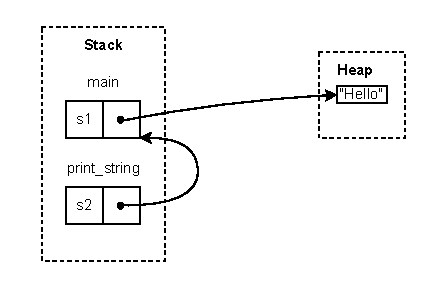
\includegraphics[scale = 1]{Figures/bor1.drawio.pdf}
    \caption{Visualizzazione memoria Rust durante la chiamata di \texttt{print\_string()}.}
    \label{fig:bor1}
\end{figure} 
In Java, non è possibile avere questo livello di indirezione, poiché i riferimenti puntano direttamente a oggetti in memoria. Infatti, il codice equivalente in Java sarebbe:
\begin{minted}[fontsize=\small]{Java}
    public class Main {
        public static void main(String[] args) {
            String s1 = "Hello";
            printString(s1); 
        }
        public static void printString(String s2) {
            System.out.println(s2);
        }
    }
\end{minted}
In questo caso, \texttt{s1} e \texttt{s2} sono entrambi riferimenti all'oggetto \texttt{"Hello"} in memoria (vedi figura \ref{fig:bor2}).
\begin{figure}[H]
    \centering
    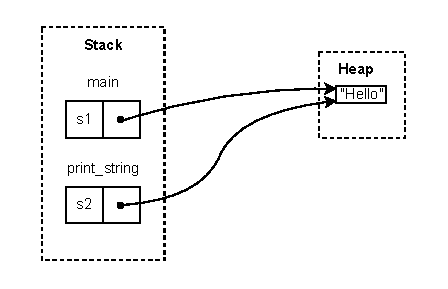
\includegraphics[scale = 1]{Figures/bor2.drawio.pdf}
    \caption{Visualizzazione memoria Java durante la chiamata di \texttt{printString()}.}
    \label{fig:bor2}
\end{figure} 
Per eseguire l'operazione opposta, ossia ottenere il valore a cui punta un riferimento, si utilizza l'operatore di dereferenziazione \texttt{*}. 

Abbiamo già visto come le variabili in Rust siano immutabili per definizione, ma è possibile dichiararle come mutabili utilizzando la keyword \texttt{mut}. I riferimenti in Rust hanno un comportamento simile: sono immutabili di default, ma possono essere dichiarati come mutabili utilizzando la keyword \texttt{mut}. Quindi, attraverso i riferimenti, è possibile accedere a un dato attraverso variabili diverse. Questo è utile per evitare la duplicazione di dati o per condividere dati tra diverse parti del programma. Tuttavia, quando si permette a più parti del codice di accedere allo stesso valore, è necessario garantire che non ci siano conflitti tra le operazioni di lettura e scrittura per evitare situazioni di errore come:
\begin{itemize}
    \item Deallocazione di un dato mentre un'altra parte del codice lo sta ancora utilizzando.
    \item Modificazione di un dato mentre un'altra parte del codice lo sta leggendo o modificando.
\end{itemize} 
In Java, i due casi sopra elencati sono permessi e la responsabilità di evitare conflitti ricade sul programmatore come già visto nell'esempio \ref{lst:java-reference}. Il problema è ancora più evidente in contesti concorrenti in cui più thread possono agire su una stessa variabile. Rust, invece, introduce un sistema di regole che impedisce questi conflitti a compile time:
\begin{itemize}
    \item Se si ha un riferimento mutabile a un valore, allora quello sarà l'unica variabile che può accedere a quel valore. Questo impedisce che una parte di codice modifichi un valore mentre un'altra parte lo sta leggendo o modificando. Se non ci sono riferimenti mutabili, allora non ci sono restrizioni sul numero di riferimenti immutabili che possono esistere contemporaneamente. 
    \item Lo scope dei riferimenti Rust inizia quando il riferimento viene creato e termina l'ultima volta che il riferimento viene utilizzato. In particolare, i riferimenti Rust non sono proprietari della variabile a cui si riferiscono, quindi quando escono dallo scope la variabile non viene deallocata.
\end{itemize}
Vediamo un esempio che mostra l'importanza di queste regole:
\begin{minted}[fontsize=\small]{rust}
    fn main() {
        let mut v = vec![1, 2, 3];
        let r1 = &v[1];
        v.push(4);
        // push prende in prestito v in modo mutabile
        // mentre r1 è un riferimento immutabile ancora attivo
        // Questo genera un errore di compilazione
        println!("Il secondo elemento e': {}", r1);
    } 
\end{minted}
Un \texttt{vec} in Rust ha un comportamento simile a un \texttt{ArrayList} in Java, ossia è un array che cresce dinamicamente. Questo significa che quando si aggiunge un elemento, il \texttt{vec} potrebbe dover allocare nuova memoria e copiare i dati esistenti in essa. Quindi, il riferimento \texttt{r1} potrebbe non puntare più al secondo elemento del \texttt{vec} dopo l'operazione \texttt{push}. Se Rust permettesse questo codice, \texttt{r1} diventerebbe un dangling pointer, cioè un riferimento non più valido\footnote{In questo codice lo scope \texttt{r1} termina dopo la sua stampa. Se non ci fosse l'istruzione di stampa non si avrebbero errori di compilazione poiché lo scope di \texttt{r1} terminerebbe dopo la sua dichiarazione}.
 Tuttavia, il compilatore impedisce questa situazione, garantendo sicurezza a tempo di compilazione.

In Java il problema dei dangling pointer è quasi inesistente, poiché i riferimenti non possono essere invalidati in questo modo. L'unico modo di ottenere un dangling pointer in Java è quello di avere un riferimento a un oggetto non inizializzato o esplicitamente impostato a \texttt{null}. Il codice equivalente in Java sarebbe:
\begin{minted}[fontsize=\small]{Java}
    public class Main {
        public static void main(String[] args) {
            List<Integer> list = new ArrayList<>();
            list.add(1);
            Integer r1 = list.get(0);
            list.add(2);
        }
    }
\end{minted}
Questo codice compila e non genera errori a run-time poiché in Java si ha un livello di indirezione in più: \text{r1} in Rust è l'indirizzo di memoria del valore "2" nel \texttt{vec}, mentre in Java è l'indirizzo di memoria dell'oggetto \texttt{Integer} che contiene il valore "2". Quindi se l'\texttt{ArrayList} venisse ridimensionato e allocato in un area di memoria diversa, ciò che viene copiato sono i riferimenti agli oggetti, non gli oggetti stessi, quindi la variabile \texttt{r1} è ancora valida perché l'oggetto a cui si riferisce non ha cambiato posizione in memoria (vedi figura \ref{fig:bor3}). 
\begin{figure}[H]
    \centering
    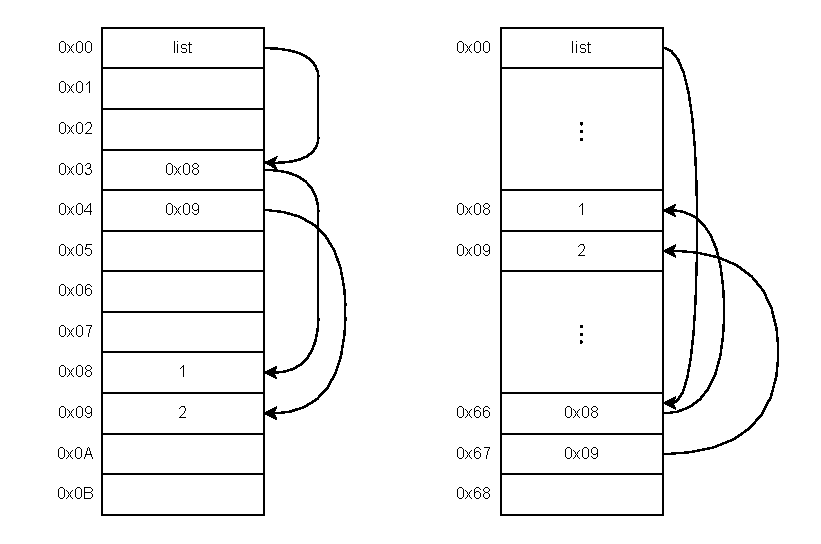
\includegraphics[width = \textwidth]{Figures/bor3.drawio.pdf}
    \caption{Memoria heap Java dopo il riallocamento dell'\texttt{ArrayList}.}
    \label{fig:bor3}
\end{figure}
\section{L'assenza di valore in Rust e Java}
In Java, il valore \texttt{null} è un concetto fondamentale che rappresenta l'assenza di un valore o un riferimento non inizializzato. Ogni riferimento a un oggetto in Java può essere impostato a \texttt{null}, indicando che non punta a nessun oggetto valido. Questo approccio, sebbene flessibile e molto potente, introduce una serie di problemi: 
\begin{itemize}
    \item \texttt{NullPointerException}: l'accesso a un metodo o a un campo di un riferimento \texttt{null} genera un'eccezione a run-time, interrompendo l'esecuzione del programma. 
    \item Ambiguità: non è chiaro se un riferimento \texttt{null} indica un errore, un valore mancante o, semplicemente, un'oggetto non  ancora inizializzato. Inoltre, può non essere ovvio se un metodo può ritornare \texttt{null} o meno, richiedendo, quindi, documentazione aggiuntiva per chiarire il comportamento atteso.
    \item Errori a run-time: problemi legati a \texttt{null} vengono rilevati solo a run-time, non durante la compilazione. 
\end{itemize}
Java cerca di mitigare questi problemi introducendo, a partire da Java 8, \texttt{Optional<T>}, un wrapper che può contenere un oggetto di tipo \texttt{T} o essere vuoto. Tramite \texttt{Optional<T>}, è possibile evitare il rischio di \texttt{NullPointerException} e rendere esplicito il fatto che un valore potrebbe non essere presente. È importante notare che, nonostante l'introduzione di \texttt{Optional<T>} e la sua crescente adozione, il problema di \texttt{null} non è completamente risolto:
\begin{itemize}
    \item \texttt{Optional<T>} non è un sostituto diretto di \texttt{null}, ma piuttosto un modo per rappresentare l'assenza di un valore in modo più sicuro. Tuttavia, codice legacy e librerie esistenti continuano a utilizzare \texttt{null}, creando un sistema duale in cui entrambi i concetti coesistono.
    \item Il compilatore Java non impone l'utilizzo di \texttt{Optional<T>} al posto di \texttt{null}. Java mette a disposizione il costrutto ma non lo impone, lasciando la scelta al programmatore, che può essere più incline a utilizzare \texttt{null} per semplicità.
    \item Anche utilizzando \texttt{Optional<T>}, è possibile incorrere in errori se non si gestisce correttamente, o, ancora peggio, non si gestisce affatto il caso in cui l'oggetto è vuoto. Ad esempio, chiamare \texttt{get()} su un \texttt{Optional<T>} vuoto solleverà un'eccezione a run-time. 
\end{itemize}
Rust, invece, elimina del tutto l'uso \texttt{null}, prevenendo molti dei problemi sopra elencati. Tuttavia, il concetto rappresentato da \texttt{null} è sempre utile. Per questo motivo, Rust adotta un approccio simile a \texttt{Optional<T>} di Java tramite il tipo \texttt{Option<T>}, definito nella libreria standard come:
\begin{minted}[fontsize=\small]{rust}
    enum Option<T> {
        Some(T), // Contiene un valore di tipo T
        None,    // Non contiene alcun valore
    }
\end{minted}
L'idea alla base di \texttt{Option<T>} è analoga a quella di \texttt{Optional<T>}: fornire una rappresentazione sicura e non ambigua dell'assenza di un valore.

\texttt{Option<T>} è un \texttt{enum} dove \texttt{Some(T)}\footnote{In Rust una variante di un \texttt{enum} può contenere uno o più valori, ognuno con il suo tipo. In questo caso \texttt{Some(T)} contiene un valore di tipo \texttt{T}.} e \texttt{None} sono le sue due varianti. La differenza principale rispetto a Java è che, poiché in Rust una variabile non può mai assumere il valore \texttt{null},per rappresentare l'assenza di valore il programmatore è costretto ad utilizzare \texttt{Option<T>}. Utilizzando la classe \texttt{Person}\footnote{Assumiamo che il campo \texttt{name} sia unico per ogni \texttt{Person}.} del listato \ref{lst:java-reference}, consideriamo il seguente esempio per mostrare l'importanza di \texttt{Option<T>} in Rust: 
\begin{listing}[h]
    \begin{minted}[fontsize=\small]{java}
    public class PersonRepository{
        private List<Person> people = new ArrayList<>();

        public Person findPersonByName(String name) {
            Objects.requireNonNull(name, "Il nome non può essere null");
            for (Person person : people) {
                if (person.getName().equals(name)) {
                    return person; // Ritorna la persona trovata
                }
            }
            return null; // Ritorna null se non trovata
        }
    }
    \end{minted}
    \caption{Utilizzo di \texttt{null} in Java.}
    \label{lst:java-optional}
\end{listing}

Il comportamento di \texttt{findPersonByName()} non risulta ovvio leggendo solo la firma del metodo e, quindi, va documentato adeguatamente. Inoltre, il chiamante deve ricordarsi di gestire il caso in cui il metodo ritorni \texttt{null}, altrimenti potrebbe incorrere in un \texttt{NullPointerException} a run-time. 

In Rust, invece, l'unico modo di avere un comportamento equivalente a quello del listato \ref{lst:java-optional} è quello di utilizzare il tipo \texttt{Option<Person>}:
\begin{minted}[fontsize=\small]{rust}
    struct Person {
        name: String,
    }

    struct PersonRepository {
        people: Vec<Person>,
    }

    impl PersonRepository {
        pub fn find_person_by_name(&self, name: &str) -> Option<&Person> {
            for person in &self.people {
                if person.name == name {
                    return Some(person); 
                }
            }
            None
        }
    }
\end{minted}
Da questo esempio\footnote{\texttt{impl} è un costrutto Rust che consente di implementare metodi per una \texttt{struct}.} si capisce come l'utilizzo di \texttt{Option<T>} renda esplicito il fatto che il metodo può non trovare una persona con il nome specificato. Inoltre, non è necessario verificare se la stringa di input \texttt{name} è \texttt{null}, poiché una variabile Rust non può essere \texttt{null}. Se si prova a passare \texttt{None} al metodo, il compilatore segnalerà un errore.

Il codice del listato \ref{lst:java-optional} può essere rifattorizzato per avere un comportamento analogo a quello di Rust, utilizzando \texttt{Optional<Person>}:
\begin{minted}[fontsize=\small]{java}
    public class PersonRepository {
        private List<Person> people = new ArrayList<>();

        public Optional<Person> findPersonByName(String name) {
            Objects.requireNonNull(name, "Il nome non può essere null");
            return people.stream()
                        .filter(person -> person.getName().equals(name))
                        .findFirst(); // Restituisce Optional<Person>
        }
    }
\end{minted}
Nonostante l'approccio di Rust risolva molti dei problemi legati a \texttt{null}, la responsabilità di utilizzare correttamente \texttt{Option<T>} ricade ancora sul programmatore. In Rust, come in Java, è necessario:
\begin{itemize}
    \item Produrre un'alternativa valida quando il valore non è presente. 
    \item Consumare il valore se è presente. 
    \item Evitare l'accesso diretto  e non controllato al valore (ad esempio \texttt{get()} in Java o, l'equivalente in Rust, \texttt{unwrap()}), poiché ciò sarebbe diverso da accedere a un valore \texttt{null}.
\end{itemize}
\begin{comment}
\section{Implementazione di una Linked List in Rust}
Per dimostrare praticamente i concetti di gestione della memoria presentati in questo capitolo, si procede con l'implementazione di una \textit{linked list} in Rust. Questa struttura dati rappresenta un caso di studio ideale poiché coinvolge direttamente i concetti di ownership, borrowing e gestione dell'assenza di valore.
\subsection{Definizione della struttura}
In Rust, una \texttt{struct} è un tipo di dato che consente di raggruppare variabili, di qualsiasi tipo, correlate. Si può pensare a una \texttt{struct} come a una classe in Java, ma senza i metodi associati. Per implementare una \textit{linked list}, si definiscono due \texttt{struct}: una per il nodo della lista e una per la lista stessa.
\begin{minted}{rust}
    // Definizione del nodo
    struct Node<T> {
        value: T,
        next: Option<Box<Node<T>>>,
    }

    // Definizione della lista
    struct LinkedList<T> {
        head: Option<Box<Node<T>>>,
    }
\end{minted}
Si utilizza l'\texttt{enum} \texttt{Option<T>} per il campo \texttt{next} per indicare che un nodo può non avere un successivo, ossia essere l'ultimo nodo della lista. L'utilizzo del tipo \texttt{Option<Box<Node<T>>>} per il campi \texttt{next} e \texttt{head} è necessario poiché una \texttt{struct} in rust deve avere una dimensione ben definita e nota a compile time. Se si utlizzasse \texttt{Option<Node<T>>}, la dimensione del tipo \texttt{Node<T>} non sarebbe limitata superiormente, poiché potrebbe crescere in maniera arbitraria a seconda della lunghezza della lista. Invece, tramite l'utilizzo del puntatatore \texttt{Box<T>} si ottiene una dimensione fissa.


    \section{Lifetimes}
    In Java, il problema dei dangling pointers non si verifica in quanto il linguaggio non prevede la deallocazione esplicita della memoria. Il garbage collector provvede automaticamente a liberare la memoria occupata dagli oggetti quando non esistono più riferimenti attivi ad essi. Di conseguenza, non è possibile avere dangling pointers, poiché un oggetto viene distrutto solo quando è effettivamente non più raggiungibile.

    Tuttavia, in Rust, poiché la memoria occupata da una variabile viene automaticamente deallocata una volta che esce dallo scope, può verificarsi una situazione in cui un riferimento alla variabile vive più della variabile stessa. Ad esempio:
    \begin{listing}[H]
        \begin{minted}[fontsize=\small]{rust}
            fn main() {
                let r;
                {
                    let s = String::from("ciao");
                    r = &s;
                } // s esce dallo scope e viene deallocato
                // r ora punta a una variabile non più valida
                println!("Il valore è: {}", r);
            }
        \end{minted}
        \caption{Tentativo di creazione di un dangling pointer in Rust.}
        \label{lst:rust-dangling-pointer}
    \end{listing}
    Per evitare questo problema, Rust utilizza un sistema di \textit{lifetimes} (durata di vita) dei riferimenti, che consente al compilatore di verificare che i riferimenti siano sempre validi durante il loro utilizzo. Il lifetime di un riferimento è definito come l'intervallo di tempo durante il quale il riferimento è valido e può essere utilizzato senza causare errori di accesso alla memoria. Nel listato \ref{lst:rust-dangling-pointer}, il riferimento \texttt{r} tenta di accedere alla stringa \texttt{s} dopo che quest'ultima è uscita dallo scope ed è stata deallocata. Il compilatore di Rust rileva questa situazione grazie all'analisi dei lifetimes e impedisce la compilazione del programma, evitando un potenziale accesso a memoria non valida. Di seguito, il codice equivalente al listato \ref{lst:rust-dangling-pointer} in Java:
    \begin{minted}[fontsize=\small]{java}
        public class Main {
            public static void main(String[] args) {
                String r;
                {
                    String s = new String("ciao");
                    r = s;
                }
                System.out.println("Il valore è: " + r);
            }
        }    
    \end{minted}
    In questo caso, anche se la variabile \texttt{s} esce dallo scope alla fine del blocco, l'oggetto "ciao" rimane in memoria perché è ancora referenziato dalla variabile \texttt{r}. Il garbage collector non interviene finché esistono riferimenti validi. Pertanto, in Java non si verifica un accesso a memoria non valida, e il programma stampa correttamente il valore.

    Nel listato \ref{lst:rust-dangling-pointer} il problema è molto semplice da risolvere: basta eliminare lo scope interno. Tuttavia, ci sono situazioni più complesse in cui non è banale determinare se un riferimento è valido o meno. 
\end{comment}
